\documentclass[tikz,border=6pt]{standalone}
\usepackage{amsmath,amssymb,mathtools,physics,bm,nicefrac,wasysym}
\usepackage{xcolor}

\definecolor{colone}{RGB}{180,60,60}
\definecolor{coltwo}{RGB}{60,110,180}
\definecolor{colthree}{RGB}{60,140,80}

\definecolor{accent}{HTML}{A13D2C}
\definecolor{accent2}{HTML}{2B5F6B}
\definecolor{muted}{HTML}{5A564F}
\definecolor{panel}{HTML}{F8F6F0}
\definecolor{linecol}{HTML}{D8D2C4}
\definecolor{ink}{HTML}{1E1C1A}
\definecolor{astroblue}{HTML}{1B4F72}
\definecolor{astrodark}{HTML}{17202A}
\definecolor{sunyellow}{HTML}{E8A33D}

\usetikzlibrary{calc,arrows.meta,positioning,decorations.pathreplacing,decorations.markings,angles,quotes,shapes.geometric}
\usepackage{tikz-3dplot}

\newcommand{\vecr}{\vec r}
\newcommand{\vecL}{\vec L}
\newcommand{\vecA}{\vec A}
\newcommand{\vecf}{\vec f}
\newcommand{\vecF}{\vec F}
\newcommand{\vecp}{\vec p}
\newcommand{\avg}[1]{\left\langle #1\right\rangle}
\newcommand{\vecx}{\vec x}
\newcommand{\hatn}{\hat n}
\newcommand{\rhat}{\hat r}
\newcommand{\phihat}{\hat\phi}
\newcommand{\thetahat}{\hat\theta}
\newcommand{\note}[1]{\textcolor{blue!60!black}{\textit{[#1]}}}

\newcommand{\LST}{\mathrm{LST}}
\newcommand{\GST}{\mathrm{GST}}
\newcommand{\GMST}{\mathrm{GMST}}
\newcommand{\GAST}{\mathrm{GAST}}
\newcommand{\LMST}{\mathrm{LMST}}
\newcommand{\LAST}{\mathrm{LAST}}
\newcommand{\UT}{\mathrm{UT}}
\newcommand{\UTC}{\mathrm{UTC}}
\newcommand{\TAI}{\mathrm{TAI}}
\newcommand{\TT}{\mathrm{TT}}
\newcommand{\TDB}{\mathrm{TDB}}
\newcommand{\JD}{\mathrm{JD}}
\newcommand{\MJD}{\mathrm{MJD}}
\newcommand{\EoT}{\mathrm{EoT}}
\newcommand{\SNR}{\mathrm{SNR}}
\newcommand{\RON}{\mathrm{RON}}



\begin{document}
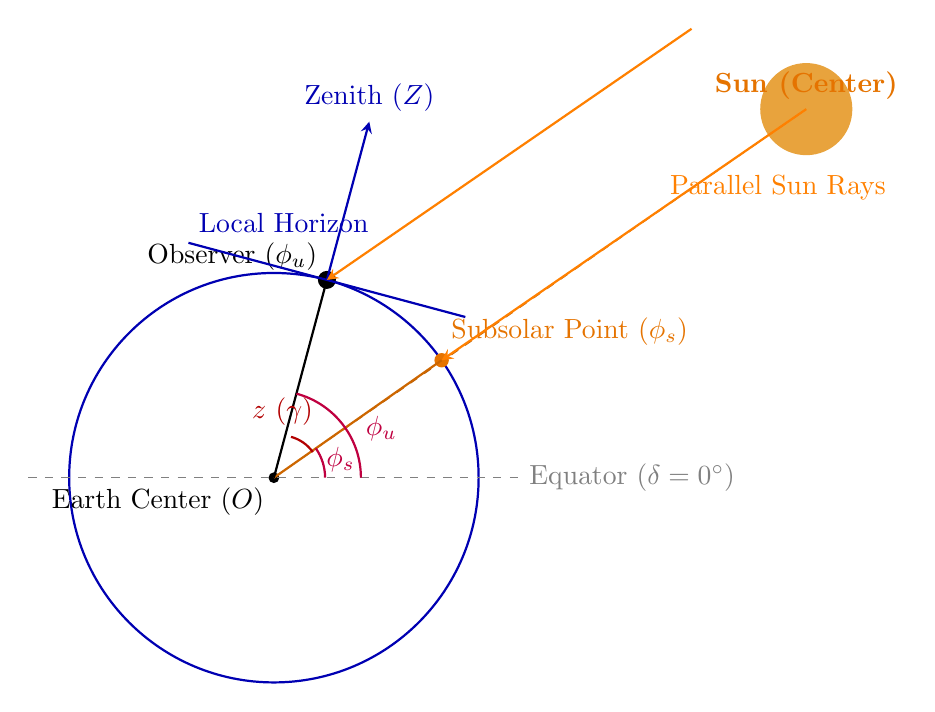
\begin{tikzpicture}[scale=1.3, >=stealth]
    		% Earth circle
    		\draw[thick, blue!70!black] (0,0) circle (2cm);
    		\fill (0,0) circle (1.5pt) node[below left] {Earth Center ($O$)};

    		% Equator line
    		\draw[dashed, gray] (-2.4,0) -- (2.4,0) node[right] {Equator ($\delta = 0^\circ$)};

    		% External Sun Icon
    		\coordinate (Sun) at (5.2, 3.6);
    		\fill[sunyellow] (Sun) circle (0.45cm);
    		\node[orange!90!black, above] at (Sun) {\textbf{Sun (Center)}};

    		% Connecting line
    		\draw[dashed, orange!70!black] (0,0) -- (Sun);

    		% Subsolar Point at intersection
    		\coordinate (Subsolar) at (35:2cm);
    		\fill[orange!90!black] (Subsolar) circle (2pt) node[above right, yshift=2pt] {Subsolar Point ($\phi_s$)};
    		\draw[thick, orange!80!black] (0,0) -- (Subsolar);

    		% Observer Position
    		\coordinate (Observer) at (75:2cm);
    		\fill[black] (Observer) circle (2.5pt) node[above left] {Observer ($\phi_u$)};
    		\draw[thick, black] (0,0) -- (Observer);

    		% Local Horizon at Observer
    		\draw[thick, blue!70!black] ($(Observer) + (-15:1.4cm)$) -- ($(Observer) + (165:1.4cm)$) node[above right] {Local Horizon};

    		% Local Zenith at Observer
    		\draw[->, thick, blue!70!black] (Observer) -- ($(Observer) + (75:1.6cm)$) node[above] {Zenith ($Z$)};

    		% Parallel Sun Ray 1
    		\draw[->, thick, orange] (Sun) -- (Subsolar);

    		% Parallel Sun Ray 2
    		\draw[->, thick, orange] ($(Sun) + (Observer) - (Subsolar)$) -- (Observer);
    		\node[orange, above right] at ($(Sun)!0.4!(Subsolar)$) {Parallel Sun Rays};

    		% Latitude angle of Subsolar point
    		\draw[thick, purple] (0.5,0) arc (0:35:0.5cm);
    		\node[purple] at (0.65, 0.18) {$\phi_s$};

    		% Latitude angle of Observer
    		\draw[thick, purple] (0.85,0) arc (0:75:0.85cm);
    		\node[purple] at (1.05, 0.48) {$\phi_u$};

    		% Zenith angle z
    		\draw[thick, red!70!black] (0.38,0.25) arc (35:75:0.38cm);
    		\node[red!70!black, above] at ($(35:0.38cm)!0.5!(75:0.38cm) + (-0.12, 0.12)$) {$z$ ($\gamma$)};
    	\end{tikzpicture}
\end{document}
